% vim: ts=2 sts=2 sw=2

\documentclass[a4paper,12pt]{report}
\usepackage[finnish]{babel}
\usepackage[utf8]{inputenc}
%\usepackage[T1]{fontenc}
\usepackage{graphicx}

\title{Levytietokanta\\
  \large{Tietokantasovellus, kevät 2011}\\}
\author{Tuomo Lempiäinen\\tuomo.lempiainen@helsinki.fi \and
Hanna Nieminen\\hanna.m.nieminen@helsinki.fi}

\begin{document}

\maketitle

\tableofcontents

\chapter{Määrittely}

\section{Johdanto}

\subsection{Järjestelmän tarkoitus}
Järjestelmän avulla sen ylläpitäjä voi pitää kirjaa omistamistaan levyistä.
Lisäksi järjestelmästä voi tehdä julkisen, jolloin myös vierailijat voivat
selata levylistaa ja yksittäisten levyjen tietoja.

\section{Yleiskuva järjestelmästä}

\subsection{Sidosryhmäkaavio}
\vspace{1em}
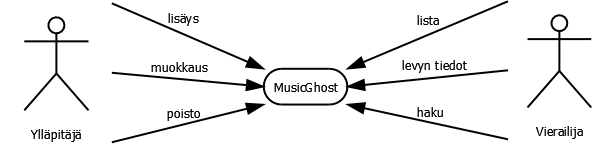
\includegraphics[width=\linewidth]{sidosryhmakaavio}

\subsection{Käyttäjäryhmät}
\begin{description}
\item[Vierailija] Kuka tahansa sivulla vieraileva käyttäjä.
\item[Ylläpitäjä] Levytietokannan omistaja, joka ylläpitää tietokantaa.
\end{description}

\section{Käyttötapaukset}

\begin{itemize}

\item Ylläpitäjä:
\begin{description}
\item[Levyn lisääminen] Ylläpitäjä voi lisätä uusia levyjä tietokantaan.
\item[Levyn tietojen muokkaaminen] Ylläpitäjä voi muokata tietokannassa olevien levyjen tietoja.
\item[Levyn poistaminen] Ylläpitäjä voi poistaa levyjä tietokannasta.
\end{description}

\item Vierailija:
\begin{description}
\item[Levylistan selaaminen] Kuka tahansa voi katsella tietokannan sisältöä.
\item[Yksittäisen levyn tietojen tutkiminen] Käyttäjä voi valita yksittäisen levyn, jolloin hänelle näytetään sen tarkat tiedot.
\item[Levyjen hakeminen hakusanalla] Käyttäjä voi antaa hakusanan, jolloin hänelle näytetään lista niistä levyistä, joiden tiedot sisältävät annetun hakusanan.
\end{description}

\end{itemize}

\end{document}
